\chapter{Introduction}
%\section{Grand Challenges For Medical Device Development}
US FDA \cite{fda} defines medical device "an instrument, apparatus, implement, machine, contrivance, implant, in vitro reagent, or other similar or related article, including a component part, or accessory which is:
\begin{itemize}
	\item recognized in the official National Formulary, or the United States Pharmacopoeia, or any supplement to them
	\item intended for use in the diagnosis of disease or other conditions, or in the cure, mitigation, treatment, or prevention of disease, in man or other animals, or
	\item intended to affect the structure or any function of the body of man or other animals, and which does not achieve any of its primary intended purposes through chemical action within or on the body of man or other animals and which is not dependent upon being metabolized for the achievement of any of its primary intended purposes."
\end{itemize}
In general, medical devices according to their risk factors for regulation purpose. In US, medical devices are categorized by FDA into 3 classes, Class I, Class II and Class III, corresponding to low-risk, medium-risk and high-risk devices \cite{class}. 
%With similar philosophy, the EU licensing process for medical devices classifies medical devices into 5 categories based on non-invasive vs. invasive, length of stay in body, contact with vessels or CNS, active vs. non-active and implantable devices. (\cite{EU_classify}) 
Devices with higher category are subject to more stringent regulations. The medical devices can also be categorized according to their applications and functions. \figref{Cur} shows example medical devices in two different classifications.
\begin{figure}[t]
		\centering
		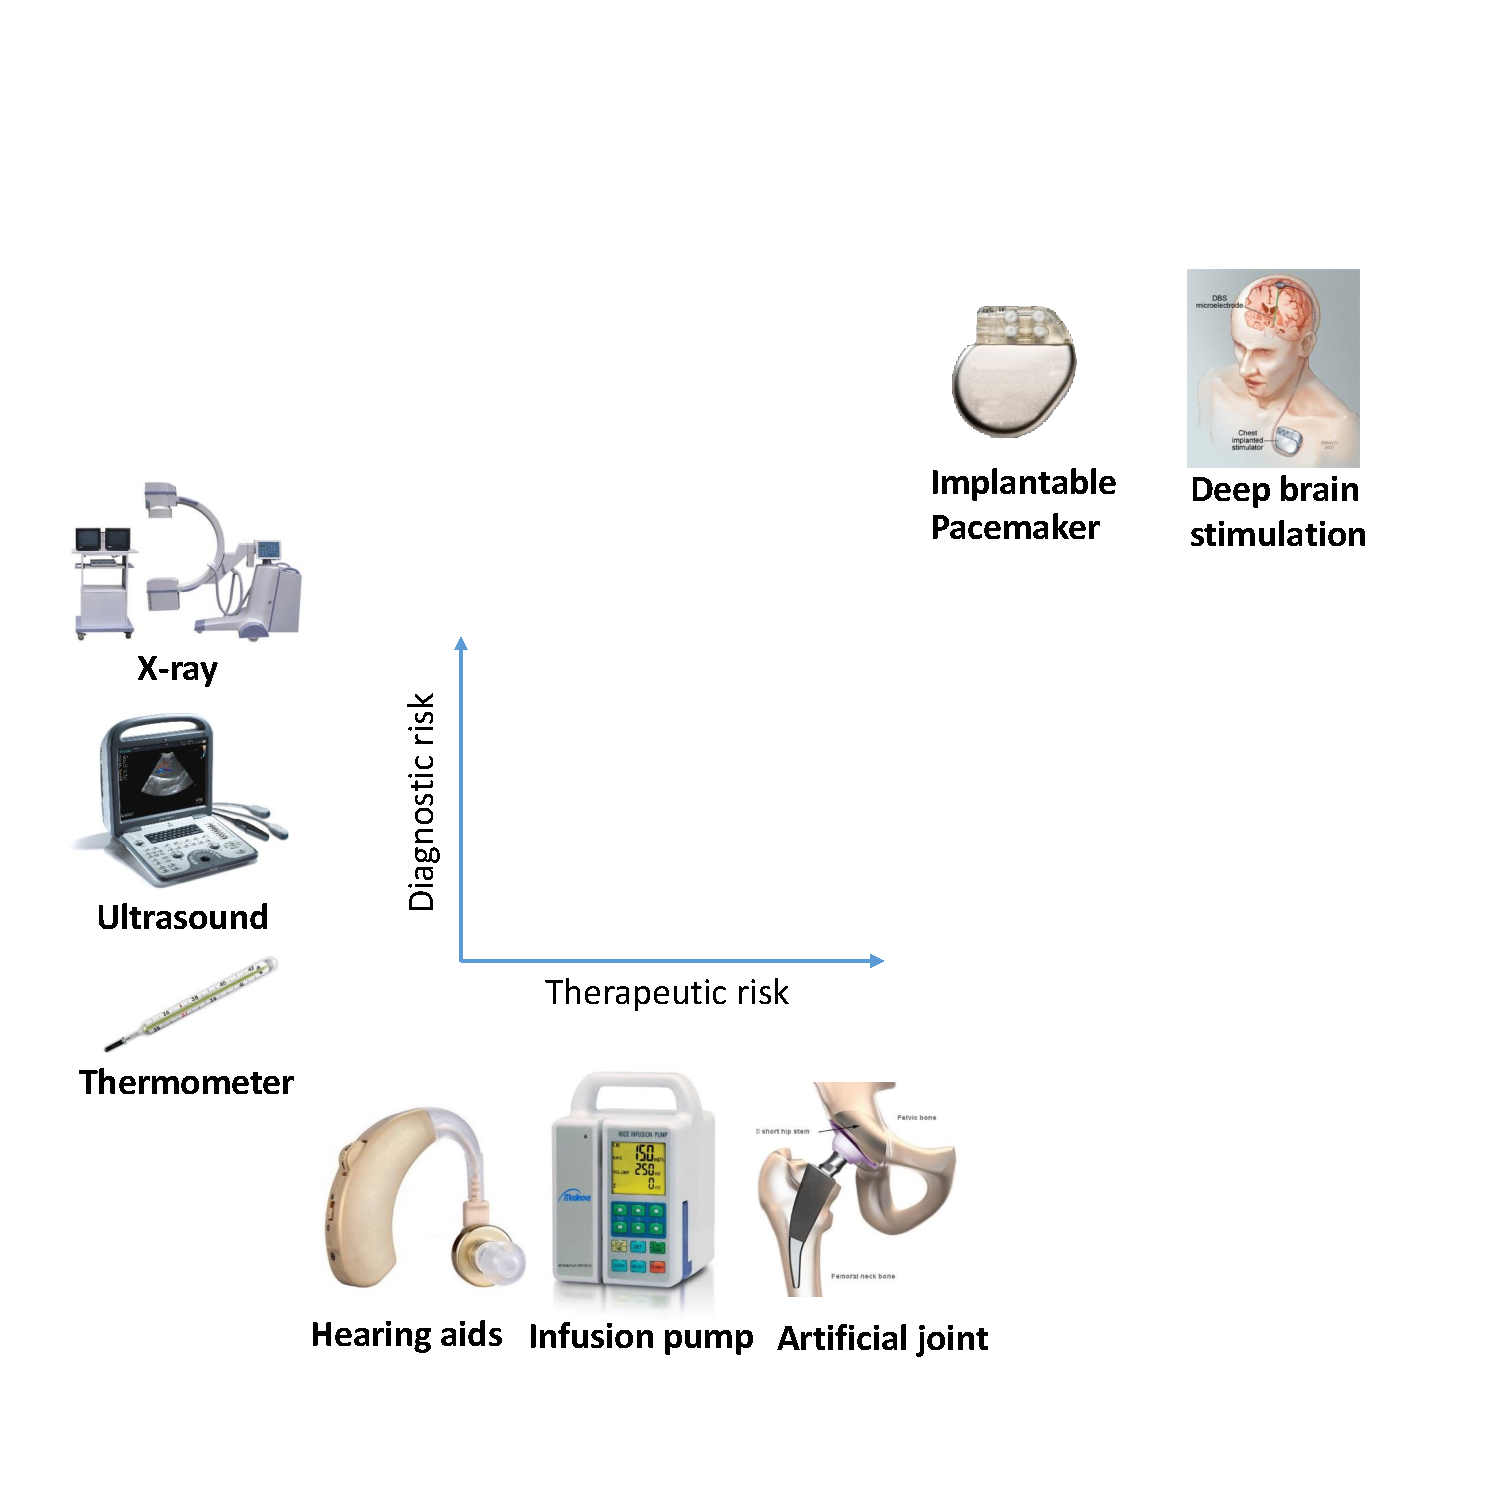
\includegraphics[width=\textwidth]{figs/devices_new.pdf}
		\caption{\small Figure of current medical devices}
		\label{fig:Cur}
\end{figure}


\section{Closing the Loop With the Patients}
Most medical devices operate with the patient in certain closed-loop manner. For diagnose-only devices, i.e. the X-ray machine, the physician operates the device to obtain patient data, perform diagnosis and deliver proper therapy to the patient (\figref{closed-loop}.(a)). For therapy-only devices, i.e. the infusion pumps, the physician operates the device to perform therapy on the patient according to previous diagnosis (\figref{closed-loop}.(b)). We denote these devices as \textbf{Open-loop Medical Devices} as there is no direct closed-loop interaction between the device and the patient. For open-loop devices, the safety of the patients is mostly guaranteed by the professionally-trained physicians in the loop. Device safety focus on providing accurate information to the physicians and faithfully operate as instructed by the physicians.

Among all the medical devices, there are devices with both diagnostic and therapeutic functions, i.e. implantable cardiac devices to treat cardiac arrhythmia, deep brain stimulation devices (\cite{Brain_sti}) to treat Parkinson's disease and artificial pancreas to treat Type 1 diabetes\footnote{The artificial pancreas is till under development by \cite{}}. These devices diagnose physiological conditions of the patient using sensory data, and deliver therapy accordingly (\figref{closed-loop}.(c)). These devices usually operate (semi-) autonomously with very little human intervention, thus malfunctions or inappropriate therapies from these devices cannot be corrected timely, which can cause serious adverse effects on patients' health. Therefore these devices are usually classified into the highest risk category and undergo the most stringent regulation. We denote them as \textbf{Closed-loop Medical Devices}. 
\begin{figure}[t]
		\centering
		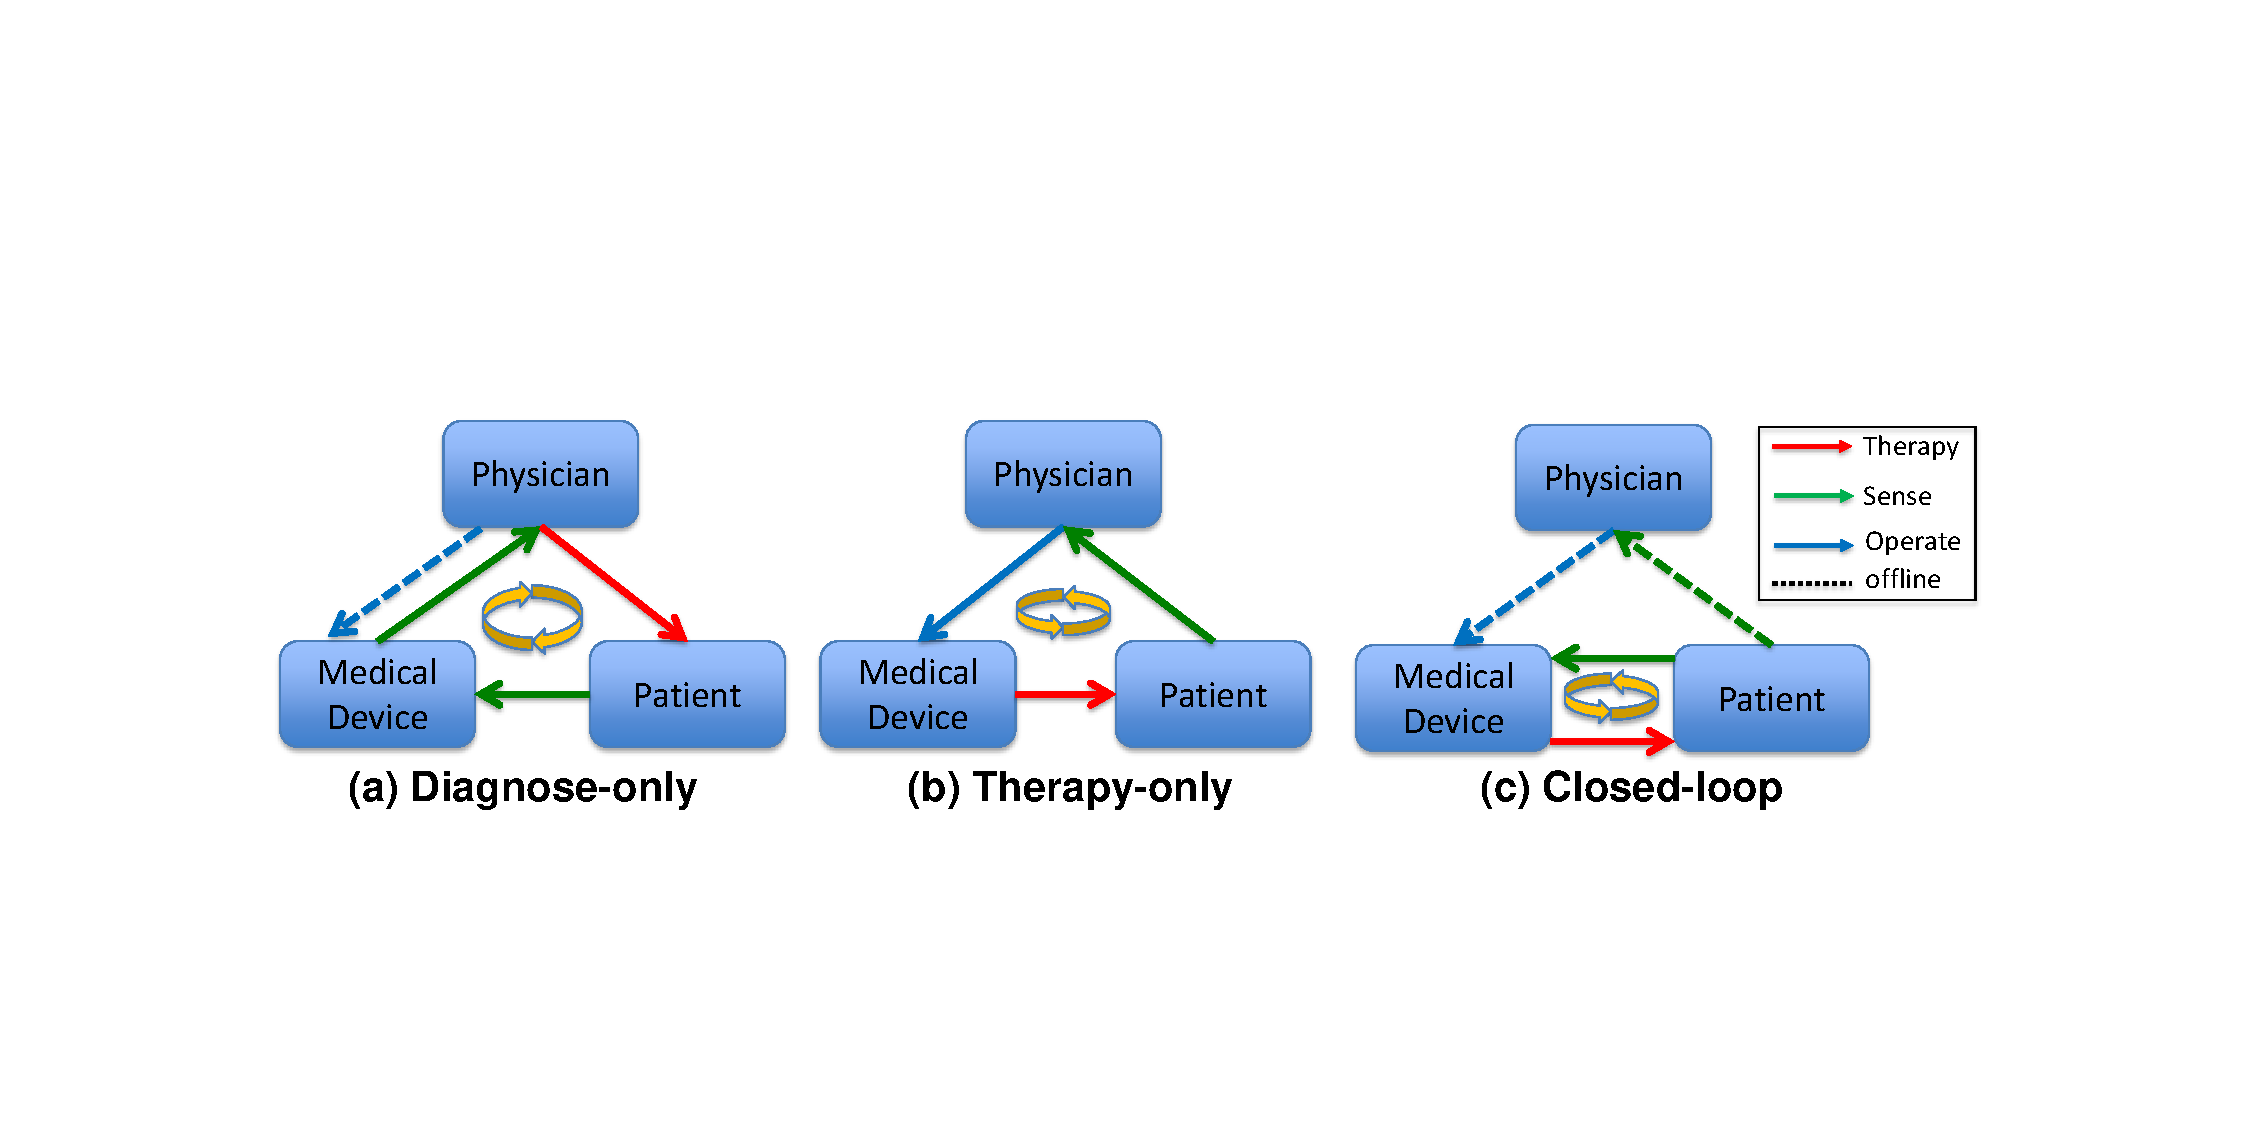
\includegraphics[width=\textwidth]{figs/closed-loop.pdf}
		\caption{\small Closing the Loop With the Patient}
		\label{fig:closed-loop}
\end{figure}
There are multiple challenges to develop safe and effective closed-loop medical devices:

\textbf{Closed-loop Interactions With Complex Physiology}\\
When using open-loop medical devices, the diagnosis and therapy decisions are made by medical professionals, who has abundant knowledge of human physiology. Therefore they are able to identify adverse health conditions and adjust the therapy accordingly. On the other hand, closed-loop medical devices have to make both the diagnosis and therapy decisions on their own. The domain expertise required to make those decisions has to be programmed into the device. It is impossible to encode all the knowledge of human physiology into the device. Therefore when conditions happen and are not programmed into the device, the device may deliver inappropriate therapy which can cause adverse effect on patient's health. 

With the development of new technology, new therapies to certain disease may arise and adopted by closed-loop devices. Certain closed-loop interactions between the device and the human physiology may not be well-understood, even to the medical professionals. Combinations of well-understood behaviors may also be the source for inappropriate therapies. In chapter \ref{ELT} we will demonstrate an example in which well-understood behaviors trigger unidentified inappropriate therapy by implantable pacemakers.

\textbf{Limited Diagnostic and Therapeutic Functions}\\
One fundamental rationale behind closed-loop medical devices is to enable the patients to live their normal lives without the dependance of cumbersome medical devices and/or the supervision of physicians. In fact, a large number of closed-loop medical devices are implantable devices. As a result, the sensing and therapy capabilities of the devices are limited, in order to increase portability and reduce invasiveness. Limited sensing capabilities may cause inaccurate diagnosis and therefore inappropriate therapy, as multiple conditions can map to the same sensor inputs. Due to limited therapy capabilities, there exists sub-optimal physiological conditions that are untreatable. The device may even trigger the conditions into less optimal conditions. In chapter \ref{mode_switch} we will demonstrate an example in which an untreatable condition is deteriorated into worse condition due to device interactions.

\textbf{Heavy Reliance on Software Control}\\\todo{I think we should not just focus on software so I put all these stats here instead of in front}
Due to the complexity of the diagnostic and therapeutic functions of the closed-loop devices, these functions are mostly controlled by their software components. 
Software embedded in a medical device, unlike electrical and mechanical components, does not fail due to corrosion, fatigue or have statistical failures of subcomponents. Software failures are uniquely sourced in the design and development of the system. %Unlike other industries such as consumer electronics where product life cycles are measured in months, software engineering for medical devices often spans a decade and must prioritize safety and efficacy over time to market. 
\begin{figure}[t]
		\centering
		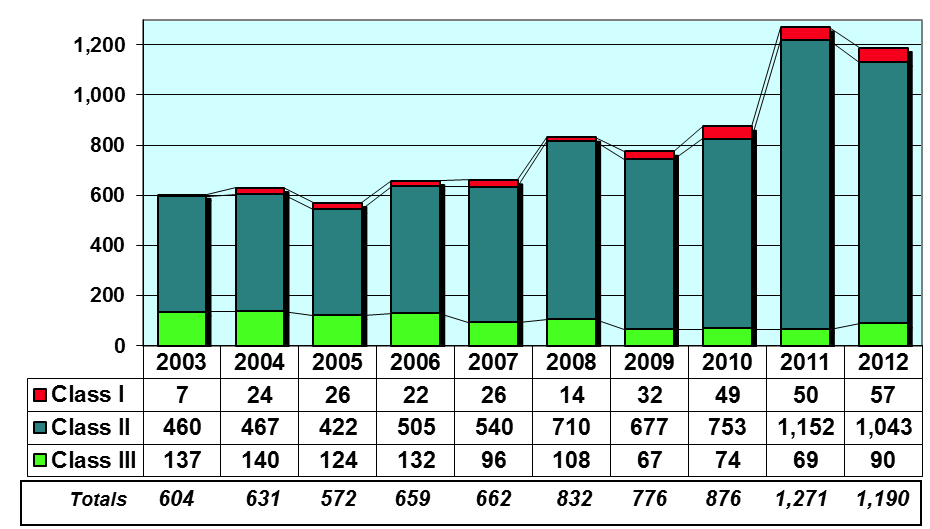
\includegraphics[width=0.8\textwidth]{figs/recalls.jpg}
		\caption{\small Figure of current medical devices}
		\label{fig:recalls}
\end{figure}
\begin{figure}[t]
		\centering
		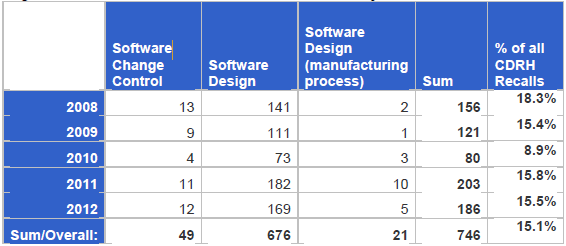
\includegraphics[width=0.8\textwidth]{figs/soft_recalls.jpg}
		\caption{\small Figure of current medical devices}
		\label{fig:soft_recalls}
\end{figure}
%  Over the course of the past four decades, cardiac rhythm management devices such as pacemakers and implantable cardioverter defibrillators (ICD) have grown in complexity and now have more than 80,000 to 100,000 lines of code (\cite{pauljones}). 
According to the US Food and Drug Administration, in 1996, 10\% of all medical device recalls were caused by software-related issues (\cite{medstats}). This percentage rose to an average of 15\% of recalls from 2008 to 2012 (\figref{soft_recalls}). Malfunctions of closed-loop medical devices usually have severe consequences, which will be categorized as \emph{Class I}, meaning there is a ``reasonable probability that use of these products will cause serious adverse health consequences or death.'' (\cite{medstats2,pacemakerrecalls,killedbycode}). 
	
\section{Regulation Efforts to Ensure Medical Device Safety}
The medical device industry is a regulated one to ensure the safety of the patients. The United States Food and Drug Administration (FDA) is the primary regulatory authority responsible for assuring the safety, efficacy and security of patients using medical devices. Based on the rationale that 1) manufacturers know their devices better than the regulator, and 2) the variety of medical devices requires a variety of approaches, the device manufacturers are responsibility to demonstrate the safety and efficacy of the medical devices. Manufacturers are required to complete pre-market submission before the devices can be released to the market. The level of requirements for the submission is determined by the safety classification of the devices. A set of general guidelines are recommended by the FDA (\cite{fda1, fda2, fda3}) which list the activities that need to be performed to ensure device safety. 

In safety-critical industries such as automotive electronics, avionics and nuclear systems, international standards are enforced for system development, evaluation, manufacturing and post-market changes (\cite{autosar,avsi}). This awareness is only beginning to enter the medical device industry as compliance with international standards are "recommended" in the aforementioned guidelines (\cite{formal_fda}). The basic rationale behind these standards is that: if all the risks/hazards of the device are identified and reasonably mitigated, and the device is developed with rigorous process, the device is reasonably safe. 

\figref{standards} demonstrates the fundamental standards to ensure medical device safety and their relationships. The IEC 60601 Medical Electrical Equipment - General requirements for basic safety and essential performance is a product safety standard that all electronic medical devices must comply to. There are emphasis on the safety of the software components. IEC 60324 specifies the processes and activities needed to perform during the software development life cycle to ensure software safety. 
Risk management is a core activity throughout the software development life cycle. ISO 14971 is specified for the application of risk management to medical devices. In addition, for each risk management activity of ISO 14971, ISO 80002-1 provides additional guidelines for the software component, which highlights and explains approaches to assuring that software safety is adequately addressed.
%The history of the FDA is a reactionary one, where each stage of evolution was in response to a major healthcare tragedy. 
\begin{figure}[t]
		\centering
		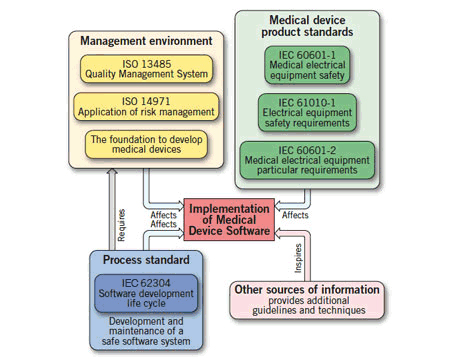
\includegraphics[width=\textwidth]{figs/standards.jpg}
		\caption{\small Figure of current medical devices}
		\label{fig:standards}
\end{figure}
\subsection{Risk Management}
Risk management includes risk analysis, risk evaluation and risk control. Fault Tree Analysis (FTA) is a common tool in risk analysis in which hazards of the system are first identified and the possible causes of the hazards are analyzed until the initial faults are reached. \figref{risks}.(a) demonstrate an example fault tree for automobile. The problem for fault tree analysis is that all possible causes are analyzed manually. In closed-loop medical devices, there may exist closed-loop interactions between the device and the patient that can cause certain hazard, but are unknown due to the limited physiological knowledge. \figref{risks}.(b) demonstrate a fault tree for a hazard of implantable pacemaker. There are several causes for undesirable fast ventricular rate. The well-understood cause is the intrinsic ventricular tachycardia (solid line). However, with pacemaker implanted, new mechanisms to cause hazard are introduced into the closed-loop system, as illustrated by the two branches with dotted lines. These two branches were not identified during the initial fault tree analysis, and were only identified after the devices have been released into the market, causing unnecessary adverse effects to the patients \cite{ELT}. Risks identified at this stage are also more costly to fix, increasing the cost for device development. \todo{Related to closed-loop model-checking}
\begin{figure}[t]
		\centering
		\includegraphics[width=\textwidth]{figs/fta_new.pdf}
		\caption{\small Figure of current medical devices}
		\label{fig:risks}
\end{figure}

After the fault tree has been constructed, probabilities for the initial faults are analyzed bottom up to calculate the probability of each hazard. The technique is called Failure Mode and Effects Analysis (FMEA). Then the risks are evaluated by assigning risk index to each hazard according to their occurrence and severity (\figref{risk_ana}). \todo{Related to requirement hierarchy}
\begin{figure}[t]
		\centering
		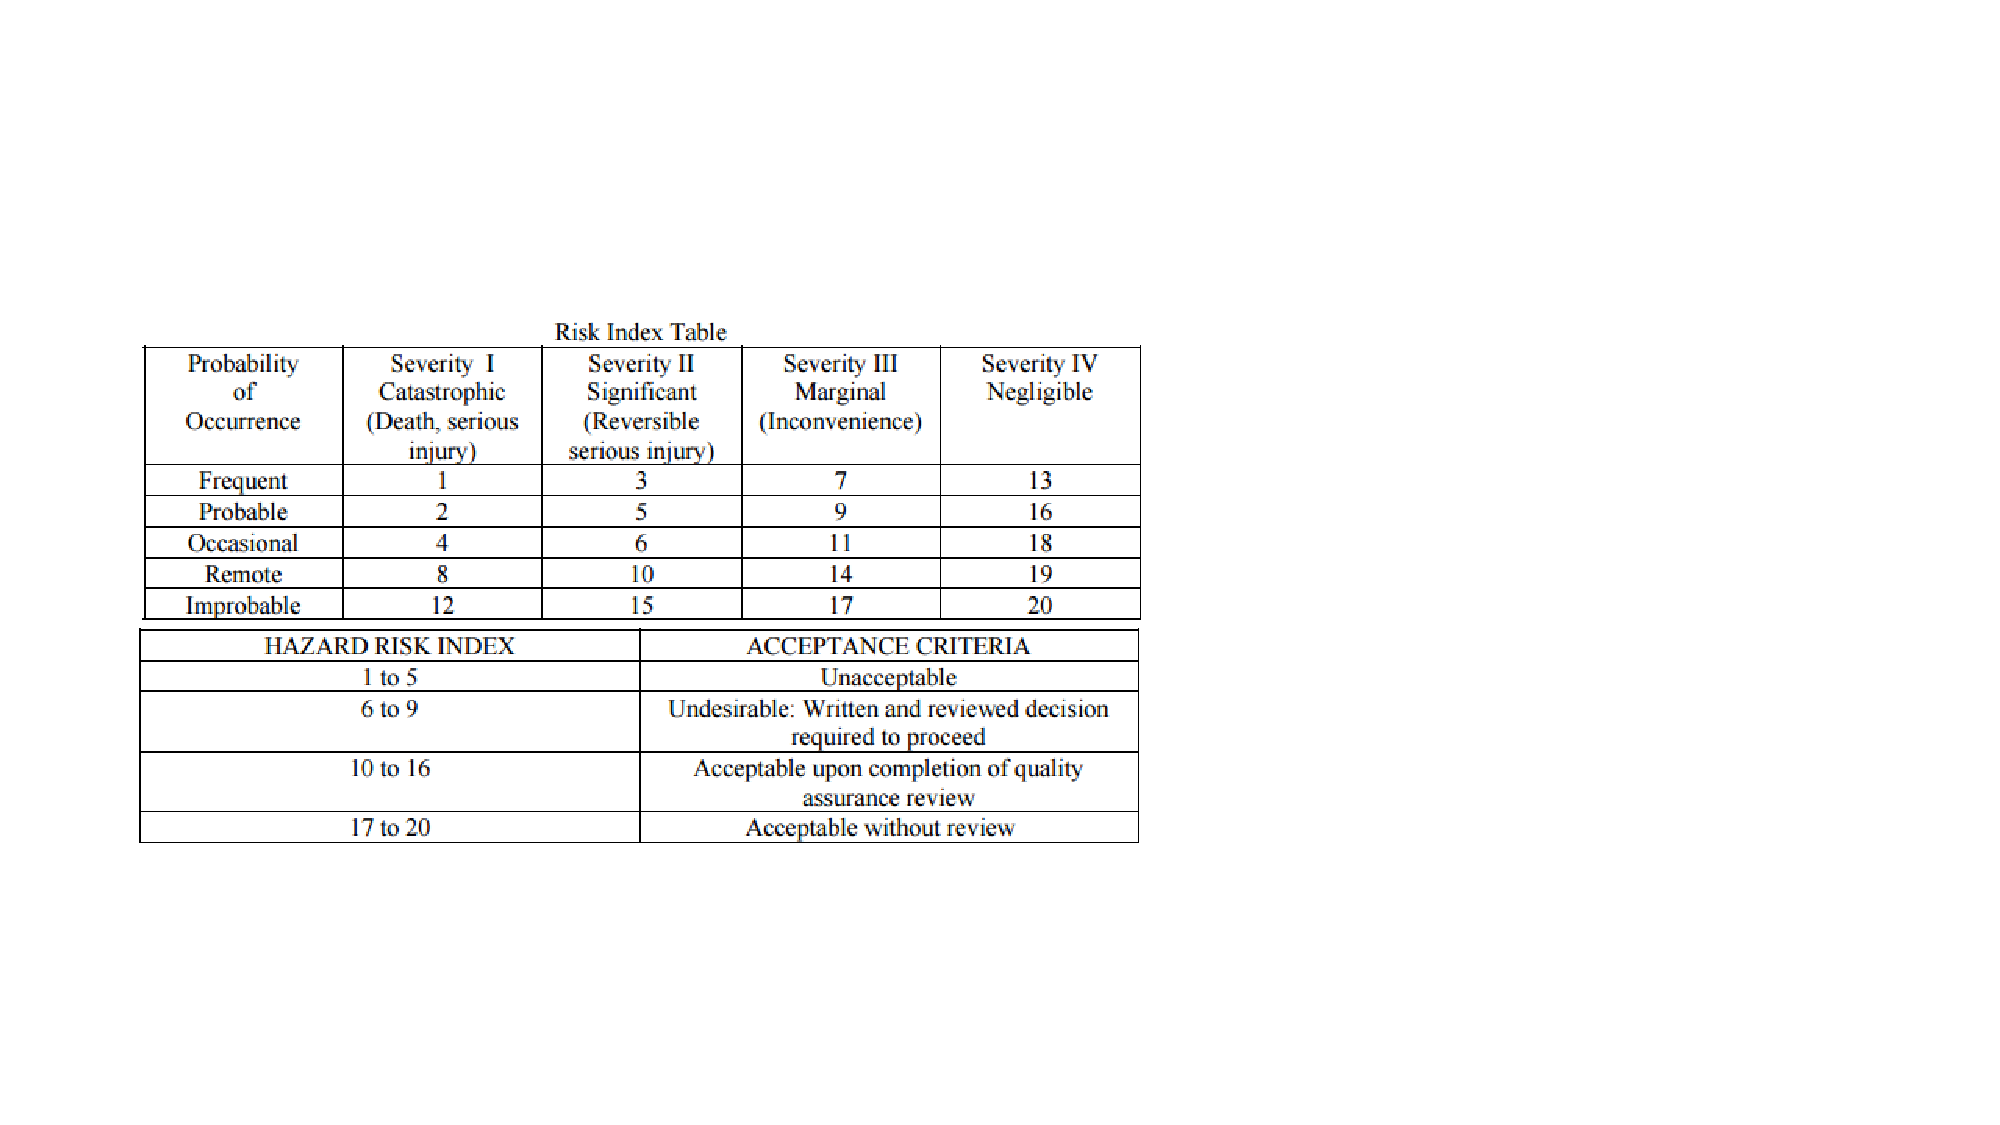
\includegraphics[width=\textwidth]{figs/risk_analysis.pdf}
		\caption{Risk analysis}
		\label{fig:risk_ana}
\end{figure}

After the risks are evaluated, different activities are required to mitigate the risks according to the risk index. After efforts made to reduce the risks, the risks should be re-evaluated to calculate the residual risk and analyze the risk/benefit. This is part of the risk control process.\todo{related to both the requirement hierarchy and model checking}
\subsection{Clinical Trials}
\todo{need some reference on this}Regardless of how rigorous the risk management and the device development process are, the devices have to be able to achieve their design goal on the real patient. Devices that have high risk factors, including the closed-loop medical devices, are required to submit clinical evidence for their safety and efficacy, often in form of clinical trials. In clinical trials the devices are used on carefully-selected group of patients following carefully designed protocols, trying to obtain unambiguous results which can support the safety and/or efficacy of the devices. 
%Through the course of the 1980s, software began to play an increasing role in medical devices. Software, as it turns out, is one of those technologies not anticipated by prior regulation, and was waiting for its disaster to prompt regulatory action. It wasn't until the 1980s when a number of cancer patients received massive X-ray overdoses during radiation therapy with the Therac-25 linear accelerator. This lead to a number of investigations, perhaps the most thorough of which was that of \cite{therac}, which was rich with identified ways software could go wrong. Inadequate testing, dangerous code reuse, configuration management issues, inadequate manufacturer response, and failure to get to the root cause of the problem were among the leaders of the problems identified. The Therac-25 was an eye-opener for the FDA and legislators, and resulted in the Safe Medical Device Act of 1990. This finally required closer medical device tracking, post-market surveillance and recommendations on development, testing and validation of medical device software. \todo{Are these useful?}

%\subsection{Pre-market Submission Process}

%There are two processes through which a medical device can enter the market in U.S.: the Premarket Notification, also known as 510(k) \cite{510k}, and the Pre-Market Approval (PMA) \cite{PMA}. In a 510(k) submission the device manufacturers are only required to provide evidence that the device is \emph{substantial equivalent} to a \emph{predicate device}, which has been approved for the market. Therefore, the 510(k) submission does not directly require clinical evidence for the safety and effectiveness of the device, thus it is suitable for mostly low-risk devices like Class I and Class II devices.  The Pre-Market Approval (PMA) submission is a more stringent regulatory process in which direct clinical evidence is required to prove the safety and effectiveness of the device. However, not all Class III devices are subject to PMA submission. If a Class III device clears the 510(k) process and FDA has not requested PMA for that device, the device is still cleared for market release. A study shows that for Class III devices which PMA has been requested, the levels of evidence varies. Only 40\% of the PMA submissions are supported by controlled clinical trials, which provide the most rigorous clinical evidence \cite{cert_prob}. The lack of quality evidence is usually due to the high cost of the controlled clinical trials.

%\subsection{Safety and Efficacy Evidence}

%\todo[inline]{List of software standards}

%The FDA currently does not request or review the medical device software during pre-market submission. This is currently satisfied by the documentation of code inspections, static analysis, module-level testing and integration testing and their purpose is to establish ``reasonable assurance of safety and effectiveness''. These tests however fail to check for the correctness of the software and are largely open-loop tests that do not consider the context of the patient. Software is reviewed by the FDA only in the incident of a device recall. Software-related recalls are often issued in the form of \emph{Safety Alerts} by the %%%%%Food and Drug Administration (FDA) 
%FDA such as ``Safety alert - Pacemaker may revert to VVI mode at 70 beats/min if programmed to one of several specific ventricular pulse widths" (\cite{medstats}).


%\section{Challenges to Develop Safe Medical Device Software}
%\subsection{Safe Development Process vs. Safe Product}
%Conformance to the safety standards provides strong confidence on a safe development process. The belief is that a well-planned, systematic engineering process produces more reliable devices, especially if software is a component of the device (\cite{med-book}). However, there is no guarantee that safe process always yield safe devices. Recently there is growing interest on enforcing safety and efficacy evidence for the device itself. \cite{Wassyng} Due to the large variety of medical devices, there does not exist general safety and efficacy requirements that can be written into standard. As the result, evidence for product safety and efficacy varies in quality and organization. Assurance cases \cite{} have been proposed to help constructing safety arguments and organizing safety evidences. Assurance cases are currently "Recommanded" by FDA during regulation submission. (\cite{})


%\subsection{Multiple Stakeholders}
%For each medical device, there are 4 stakeholders: the regulator, the device manufacturer, the medical professional and the patient. All parties have the incentive to ensure the safety and efficacy of the device. With current regulation framework, the evidence for safety 
%\begin{figure}[t]
		%\centering
		%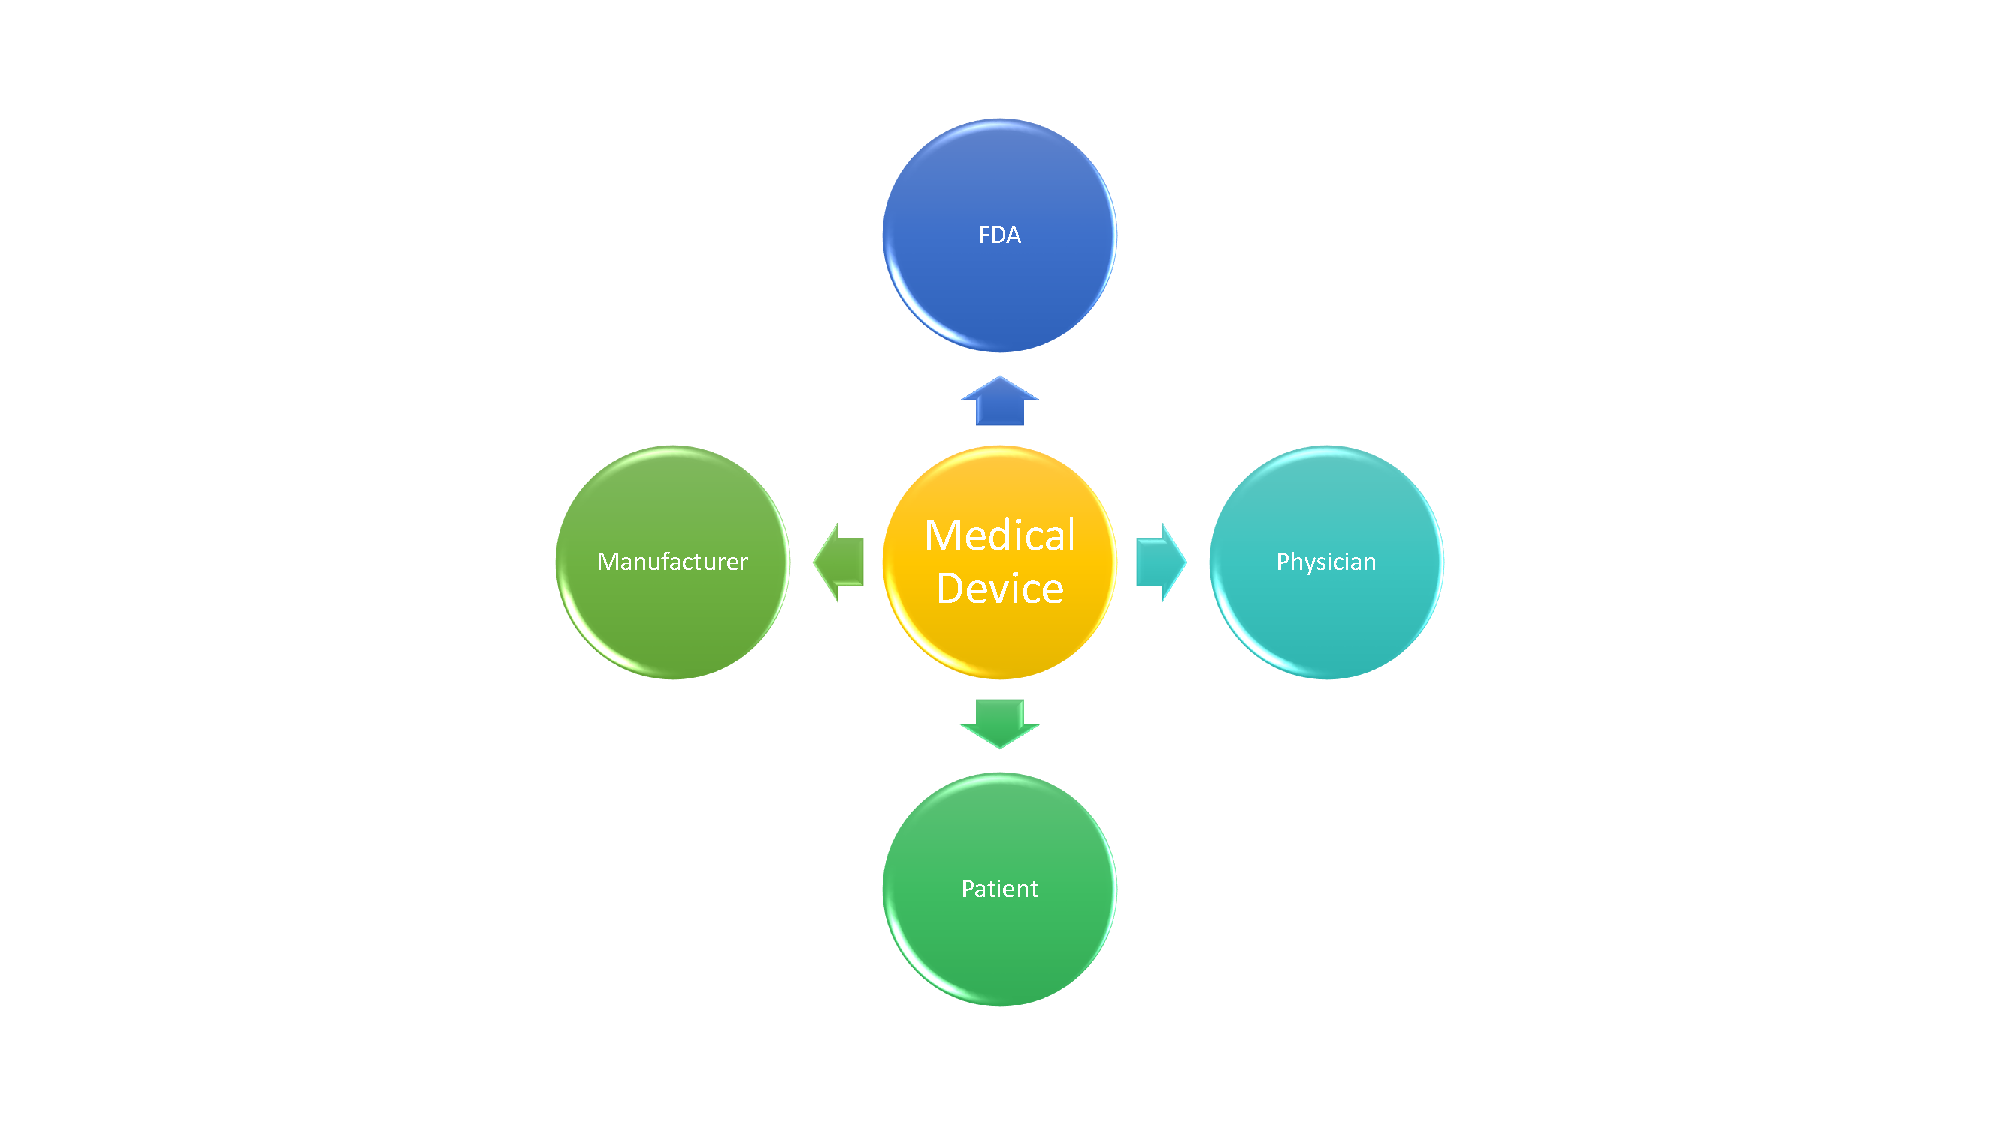
\includegraphics[width=0.8\textwidth]{figs/stakeholders.pdf}
		%\caption{\small Figure of current medical devices}
		%\label{fig:Cur}
%\end{figure}
%However, the medical domain presents its own unique set of challenges:\\
%\textbf{1. Closed-loop context:} Current evaluation of devices is open-loop and is unable to ensure the device never drives the patient into an unsafe state. Medical device testing and validation must thus be within the closed-loop context of the patient physiology. The context of the patient is a function of both the environment and the input from the device controller and must be captured by the device evaluation process.\\ 
%\textbf{2. Patient models:} There is a scarcity of patient models and clinically-relevant simulators for device design (\cite{pat-model}). High-fidelity models of interaction between the patient and device are needed to evaluate the safety and efficacy of device operation. Furthermore, these models must integrate the functional and formal aspects so that testing and verification are evaluated for the same patient states.\\
%\textbf{3. Adaptive patient-specific algorithms:} The therapy offered by the device must adapt to the environment and specific patient's condition. There is a need for validation algorithms to ensure that device control and optimization can cover large classes of patient conditions. 

%\section{The FDA and Medical Device Software}
%Before we delve into the current state of medical device software, it is useful to understand the evolution of the regulatory environment. 




%\section{Current Testing, Validation and Verification Approaches}
%In order to facilitate the early detection and correction of any software defects, the FDA has focused on infusion pumps due to the large number of recalls. In April 2010, the FDA began the ``Infusion Pump Improvement Initiative" which offers manufacturers ``the option of submitting the software code used in their infusion pumps for analysis by agency experts prior to premarket review of new or modified devices." 	\cite{}
%
%An effective software verification methodology is therefore needed for the risk analysis and certification of medical device software during the pre-market submission phase. While formal methods of verification are used for medical device software (\cite{challenge, challenge2, challenge3}), testing continues to be required because it can expose different kinds of problems (e.g. compiler bugs), can examine the program in its system context, and increases the diversity of evidence available. Testing for medical device software currently is ad hoc, error prone, and very expensive. Traditional methods of testing do not suffice as the test generation cannot be done independently of the current state of the patient and organ. The primary approach for system-level testing of medical devices is unit testing using a playback of pre-recorded electrogram and electrocardiogram signals (\cite{testing_imd, Vip}). This tests if the input signal triggers a particular response by the pacemaker, but has no means to evaluate if the response was appropriate for the patient condition. Furthermore, this approach of ``tape testing''\Hao{elaborate} is unable to check for safety violations due to inappropriate stimulus by the pacemaker. Pacemaker Mediated Tachycardia (PMT), a condition that is described later in this paper, is a strong example of why we need a model of the heart such as the one presented in this paper, which can be used for closed-loop system analysis. 
%PMT is a condition where the pacemaker inappropriately drives the heart-rate toward the upper rate limit. With a tape test, PMT would not occur and the response of the pacemaker could be classified as appropriate therapy.
%\begin{figure}[t]
		%\centering
		%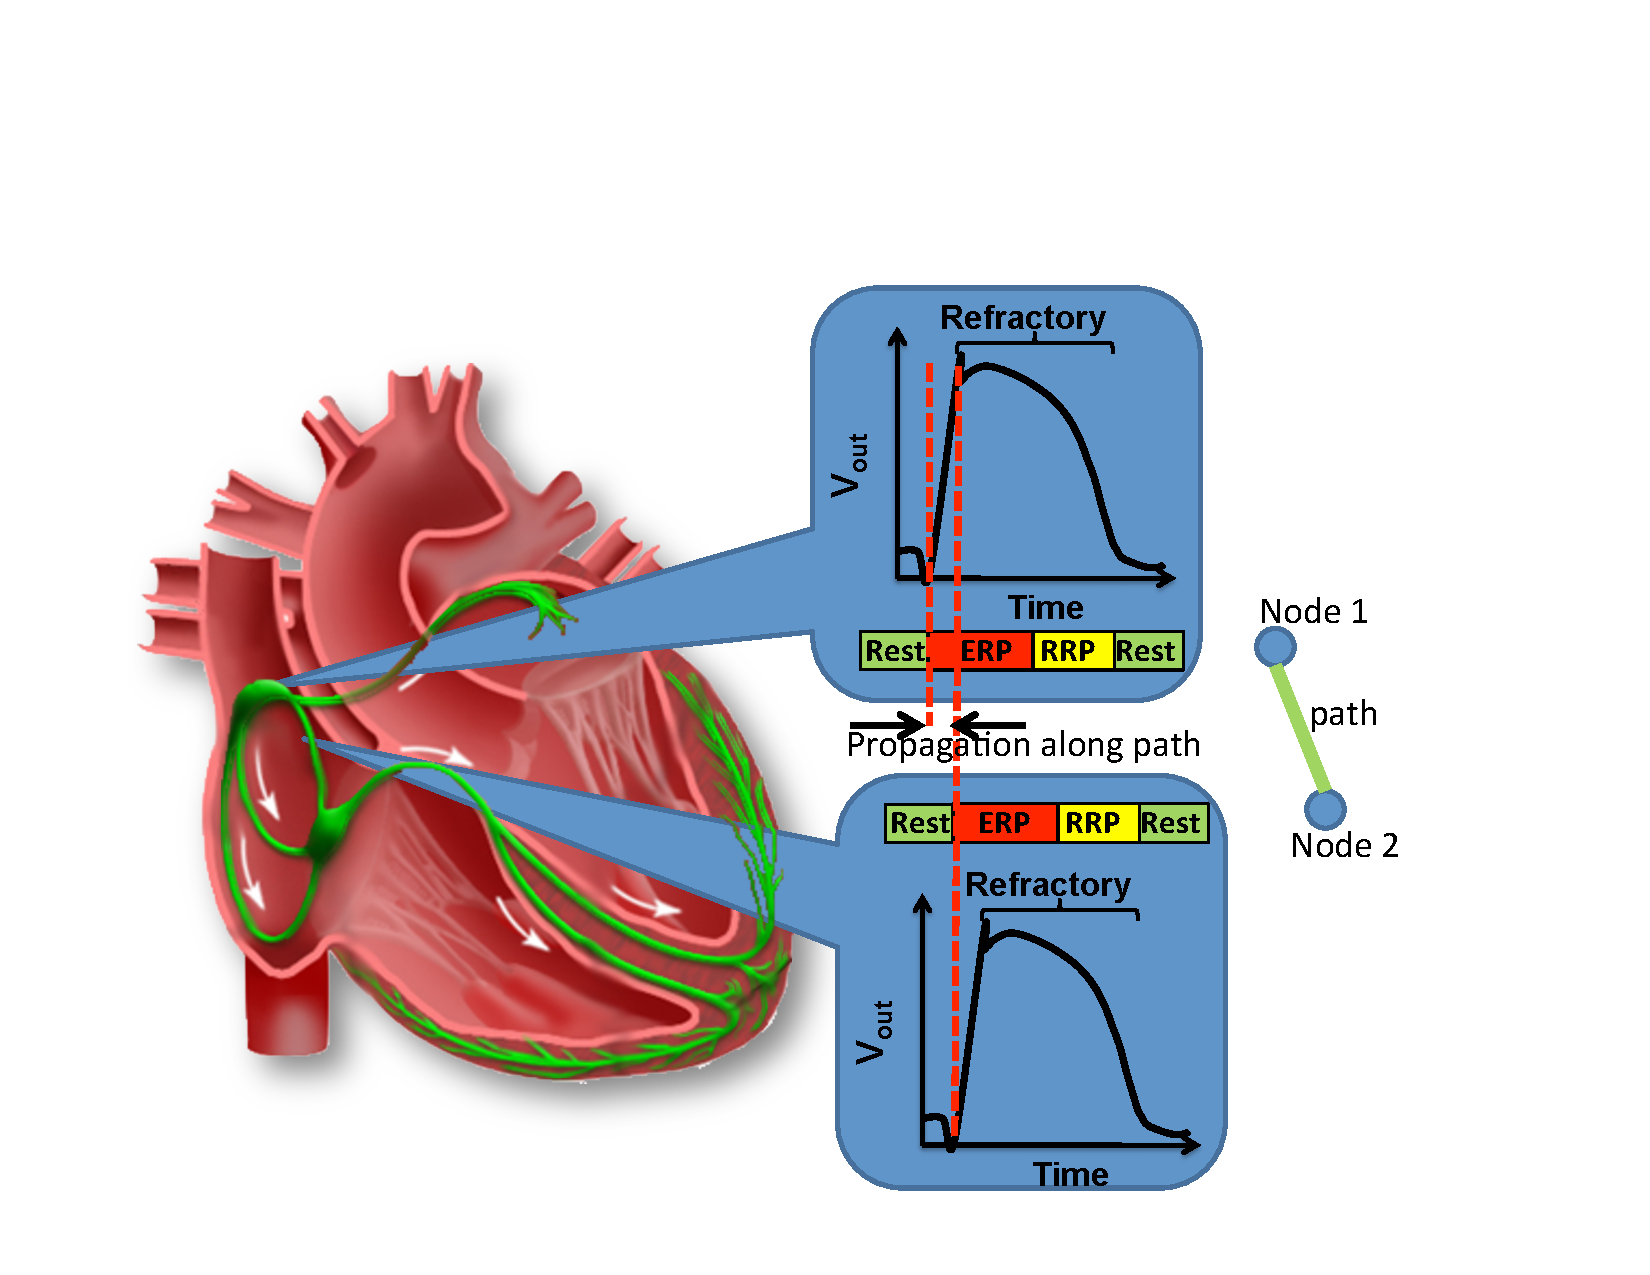
\includegraphics[width=0.8\textwidth]{figs/heartmodel.pdf}
		%%\vspace{-5pt}
		%\caption{\small By extracting timing and electric conduction information we model the signal activation, refractoriness and propagation across the heart tissue as a set of node and path automata.}
		  %%\vspace{-15pt}
		%\label{fig:heartmodel}
%\end{figure}
%As the testing environment (i.e., patient condition) is not entirely under the control of the tester, the problem changes significantly as a degree of nondeterminism is introduced in the process. Implantable medical devices are a primary example of Medical Cyber-Physical Systems where the safety and efficacy of the device and device software must be evaluated within a closed-loop context of the patient. The key challenge is in the generation of physiologically relevant tests such that the device does not provide inappropriate therapy, and does not adversely affect the safety of the patient. In addition, test generation must be interactive and adaptive such that the previous test stimulus affects the current state of the patient. The test generator must consider the current state when generating the next input in a way that advances the purpose of the test. The problem becomes one of the controller synthesis problems and cannot be addressed by an off-the-shelf model checker~\cite{rushby}.  
   %
%Formal methods have traditionally been used for verification of time-critical and safety-critical embedded systems \cite{form-meth}. Until recently, these methods have not been used for medical device certification. \cite{med-form3} presented the use of Extended Finite State Machines for model checking of a resuscitation device. Formal techniques have also been applied to improve medical device protocols (\cite{med-form2}) and safety (\cite{med-form1}), but the authors either used a simplified patient model or did not model the patient at all. 
\section{Improve Medical Device Safety with Model-based design}
Conducting clinical trials is very time consuming and expensive and risks found during clinical trials are very expensive to fix. Model-based design can potentially help during the development process and provide extra confidence to the device before conducting clinical trials. Computer models of human physiology have been developed which enable model-based closed-loop evaluations of the closed-loop medical devices. FDA is starting to recognize model simulation results as evidence for device safety and effectiveness. \cite{pancreas_paul} developed glucose-insulin models that can be used to evaluate control algorithms for artificial pancreas devices which can sense blood glucose and deliver insulin. Simulation results with the models have been recognized by FDA to replace animal trials, which significantly reduced cost (\cite{pancreas}).

In this paper we use implantable pacemaker as example to demonstrate how model-based design can help improve the safety and efficacy of the implantable pacemaker during software development. We demonstrate the development process from the perspective of the verification team of device manufacturers, therefore we assume to have full access to the pacemaker software design. The pacemaker software design is referenced from a dual chamber pacemaker from Boston Scientific (\cite{compass}).

Our proposed model-driven design (MDD) for closed-loop medical devices begins with developing heart models that can interact with real and modeled pacemakers (\cite{VHM_proc}). With the help of heart models, hazards themselves can be used as requirements directly and identify known and even unknown mechanisms that may trigger the hazards using techniques like model checking.

\todo{We may need to make another figure since this one does not show clearly how those activities fits in regulation}
As shown from the top of \figref{modeling_overview}, the heart-pacemaker closed-loop systems is first modeled abstractly to facilitate verification of the basic pacemaker design with maximum coverage (\cite{STTT13}). In our case, we use timed automata and the UPPAAL model checker at this design stage.

Next, the models are translated to more detailed models that take into account the complex dynamics of the heart and interaction with more detailed pacemaker model (\cite{vhm_ecrts10, vhm_embc11,vhm_iccps11}). We use Stateflow and Simulink at this design stage. These models are validated by physicians for their clinical relevance. The automatic model translation procedure, from UPPAAL to Stateflow, ensures that abstract models used for verification over-approximate the more detailed models used downstream (\cite{RTAS12}). Once the detailed models pass simulation-based testing with closed-loop dynamics, they are automatically generated into code and are subject to platform-level integration testing (\cite{vhm_website}). This MDD approach ensures the closed-loop safety properties are retained through the design toolchain and facilitates the development of verified software from verified models.
\begin{figure}[t]
		\centering
		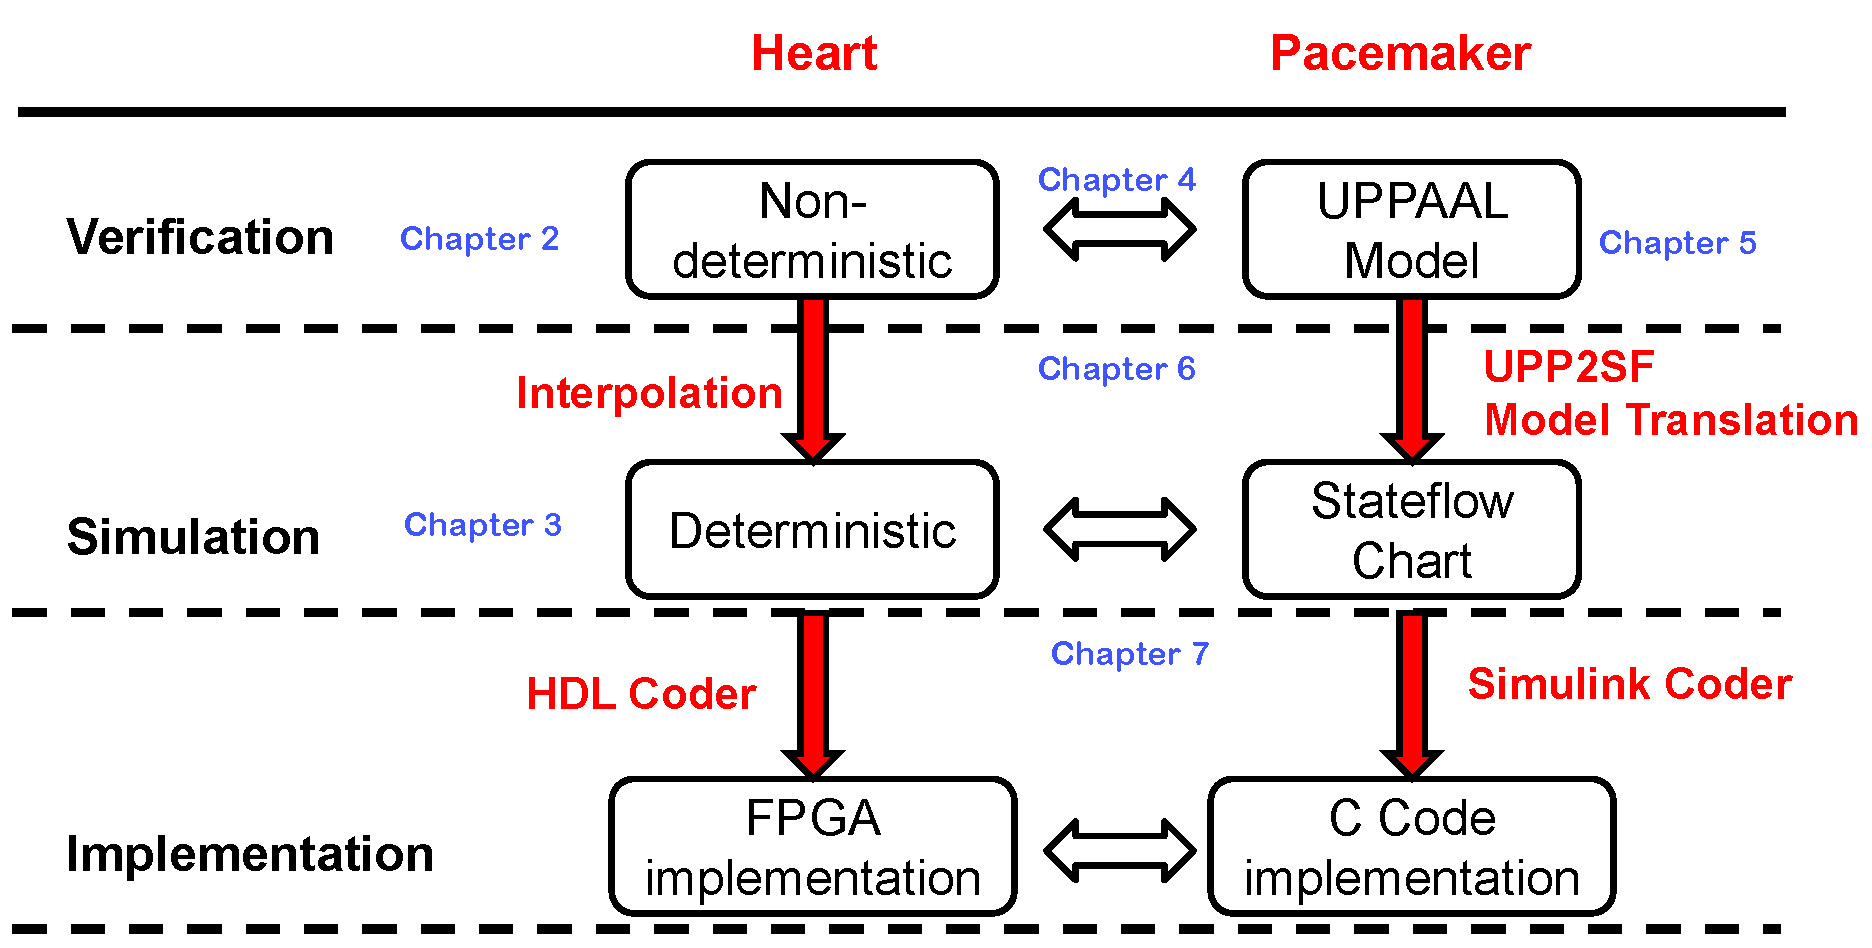
\includegraphics[width=0.8\textwidth]{figs/modeling_overview.jpg}
		%\vspace{-5pt}
		\caption{\small Model-driven design for verified models to verified code for the closed-loop heart and pacemaker system}
		  %\vspace{-15pt}
		\label{fig:modeling_overview}
\end{figure}

The focus of this effort is three-fold: (a) We developed an integrated functional (i.e., clinically-relevant) and formal (i.e., timed automata based) Virtual Heart Model  (VHM) (see \figref{heartmodel}) and a pacemaker device model for interactive and clinically relevant test generation.  (b) We provide a set of general and patient condition-specific pacemaker software requirements to ensure the safety of the patient is met under all cases, and (c) We provide a means to test and verify the closed-loop system over a variety of basic operation tests where the heart rate must be maintained, the atrial-ventricle synchrony must be enforced and complex closed-loop tests, where the pacemaker must not initiate tachycardia or perform improperly during lead displacement. With this approach of model-based testing, an executable functional model of the pacemaker is created at an early stage in the development process. This model-based methodology is an early step in addressing the urgent need for pre-market evaluation of medical device design and certification.


\section{Terminologies}
\todo{Should this come before or after the contribution section? it seems that the contributions have a good continuation from the problems}
Ensuring the safety of complex medical devices has drawn interest not only from stakeholders like regulators and industries, but also medical professionals and academia. Different communities have different interpretations over certain terminologies, causing misunderstandings. In this paper we adopt the terminologies from the regulation perspective, so that the results we have fit into the regulation framework. Most of the definitions are referred from the FDA guideline document General Principles of Software Validation (\cite{fda2}). Below are several terminologies that we use throughout the paper which worth clarifying.
\subsection{Requirements vs. Specifications}
By the definition of FDA (\cite{fda3}), the requirements of a system specify \textbf{what} the system should achieve and the specifications of a system specify \textbf{how} the system is designed to satisfy the requirements. For example, a requirement for an automobile is "Car should not hit objects". The corresponding specification can be "brake if the speed of the car is $x$ and the distance to the object is $y$". From the example we can see that a car satisfying its specification may not satisfy the requirement. In this paper, we use the word requirement in particular to denote the intended uses of the medical devices to improve physiological conditions.

\subsection{Validation vs. Verification vs. Testing}
As defined in \cite{fda2}, software validation is the confirmation by examination and provision of objective evidence that:
\begin{enumerate}
	\item software specifications conform to user needs and intended uses, and that
	\item the particular requirements implemented through software can be consistently fulfilled
\end{enumerate}
The first aspect ensures the device is safe and effective. The second aspect maintains the traceability of requirements throughout the development life cycle.
Software verification fulfills the second aspect of software validation by "providing objective evidence that the design outputs of a particular phase of the software development life cycle meet all of the specified requirements for that phase. "
\begin{figure}[t]
		\centering
		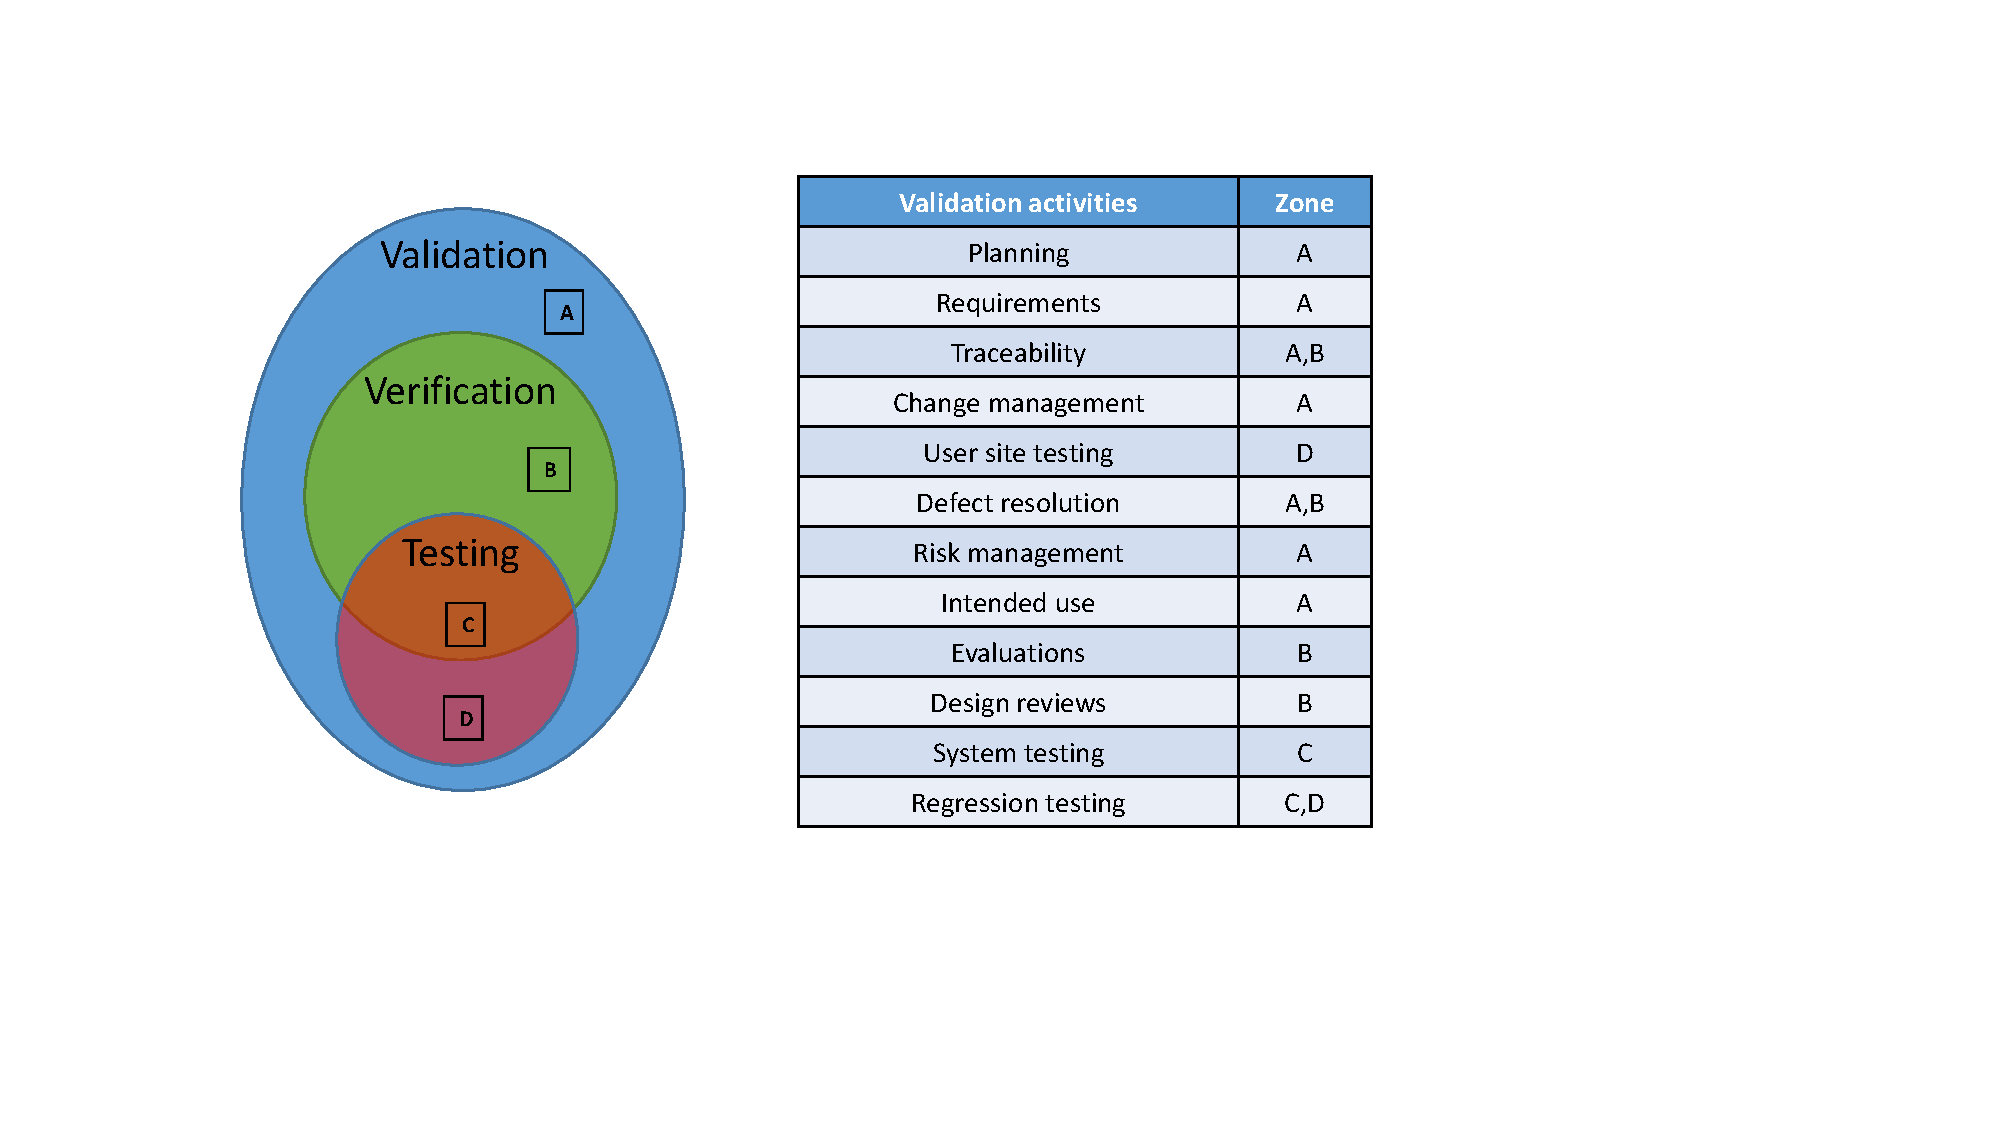
\includegraphics[width=\textwidth]{figs/validation.pdf}
		\caption{Validation activities during the software development life cycle (\cite{Vogel})}
		\label{fig:validation}
\end{figure}
Testing is the techniques that can be used for validation and/or verification. \figref{validation} illustrates the relationship between validation, verification and testing, and different activities during the software development life cycle to ensure the safety and effectiveness of the software.
\subsection{Closed-loop vs. Open-loop Evaluation}
In open-loop evaluation, i.e. open-loop testing, input sequences are send to the system and system outputs are compared with expected outputs. In open-loop testing, the system outputs do not affect the inputs afterward. In closed-loop evaluation, the environment of the system is taken into account. System outputs affect the state of the environment and thus affect the input sequences. For closed-loop medical devices, clinical trials are currently the most common closed-loop evaluation method. Enable closed-loop evaluation at model level requires models of the environment, which is human physiology for closed-loop medical devices.

Closed-loop evaluation does two things in model-based design 1) Enforce environmental constraints so that the test space is smaller and the test cases are physiological relevant. 2) Execution traces can be better interpreted as the physiological models encode domain knowledge. 
%%Through each of the chapters to follow, we cover different aspects of modeling the physiological system and the device, validating the models, running model checking on the closed-loop system and testing the deterministic systems derived from the abstract models. With the goal of 
